\begin{figure}
    \begin{center}
    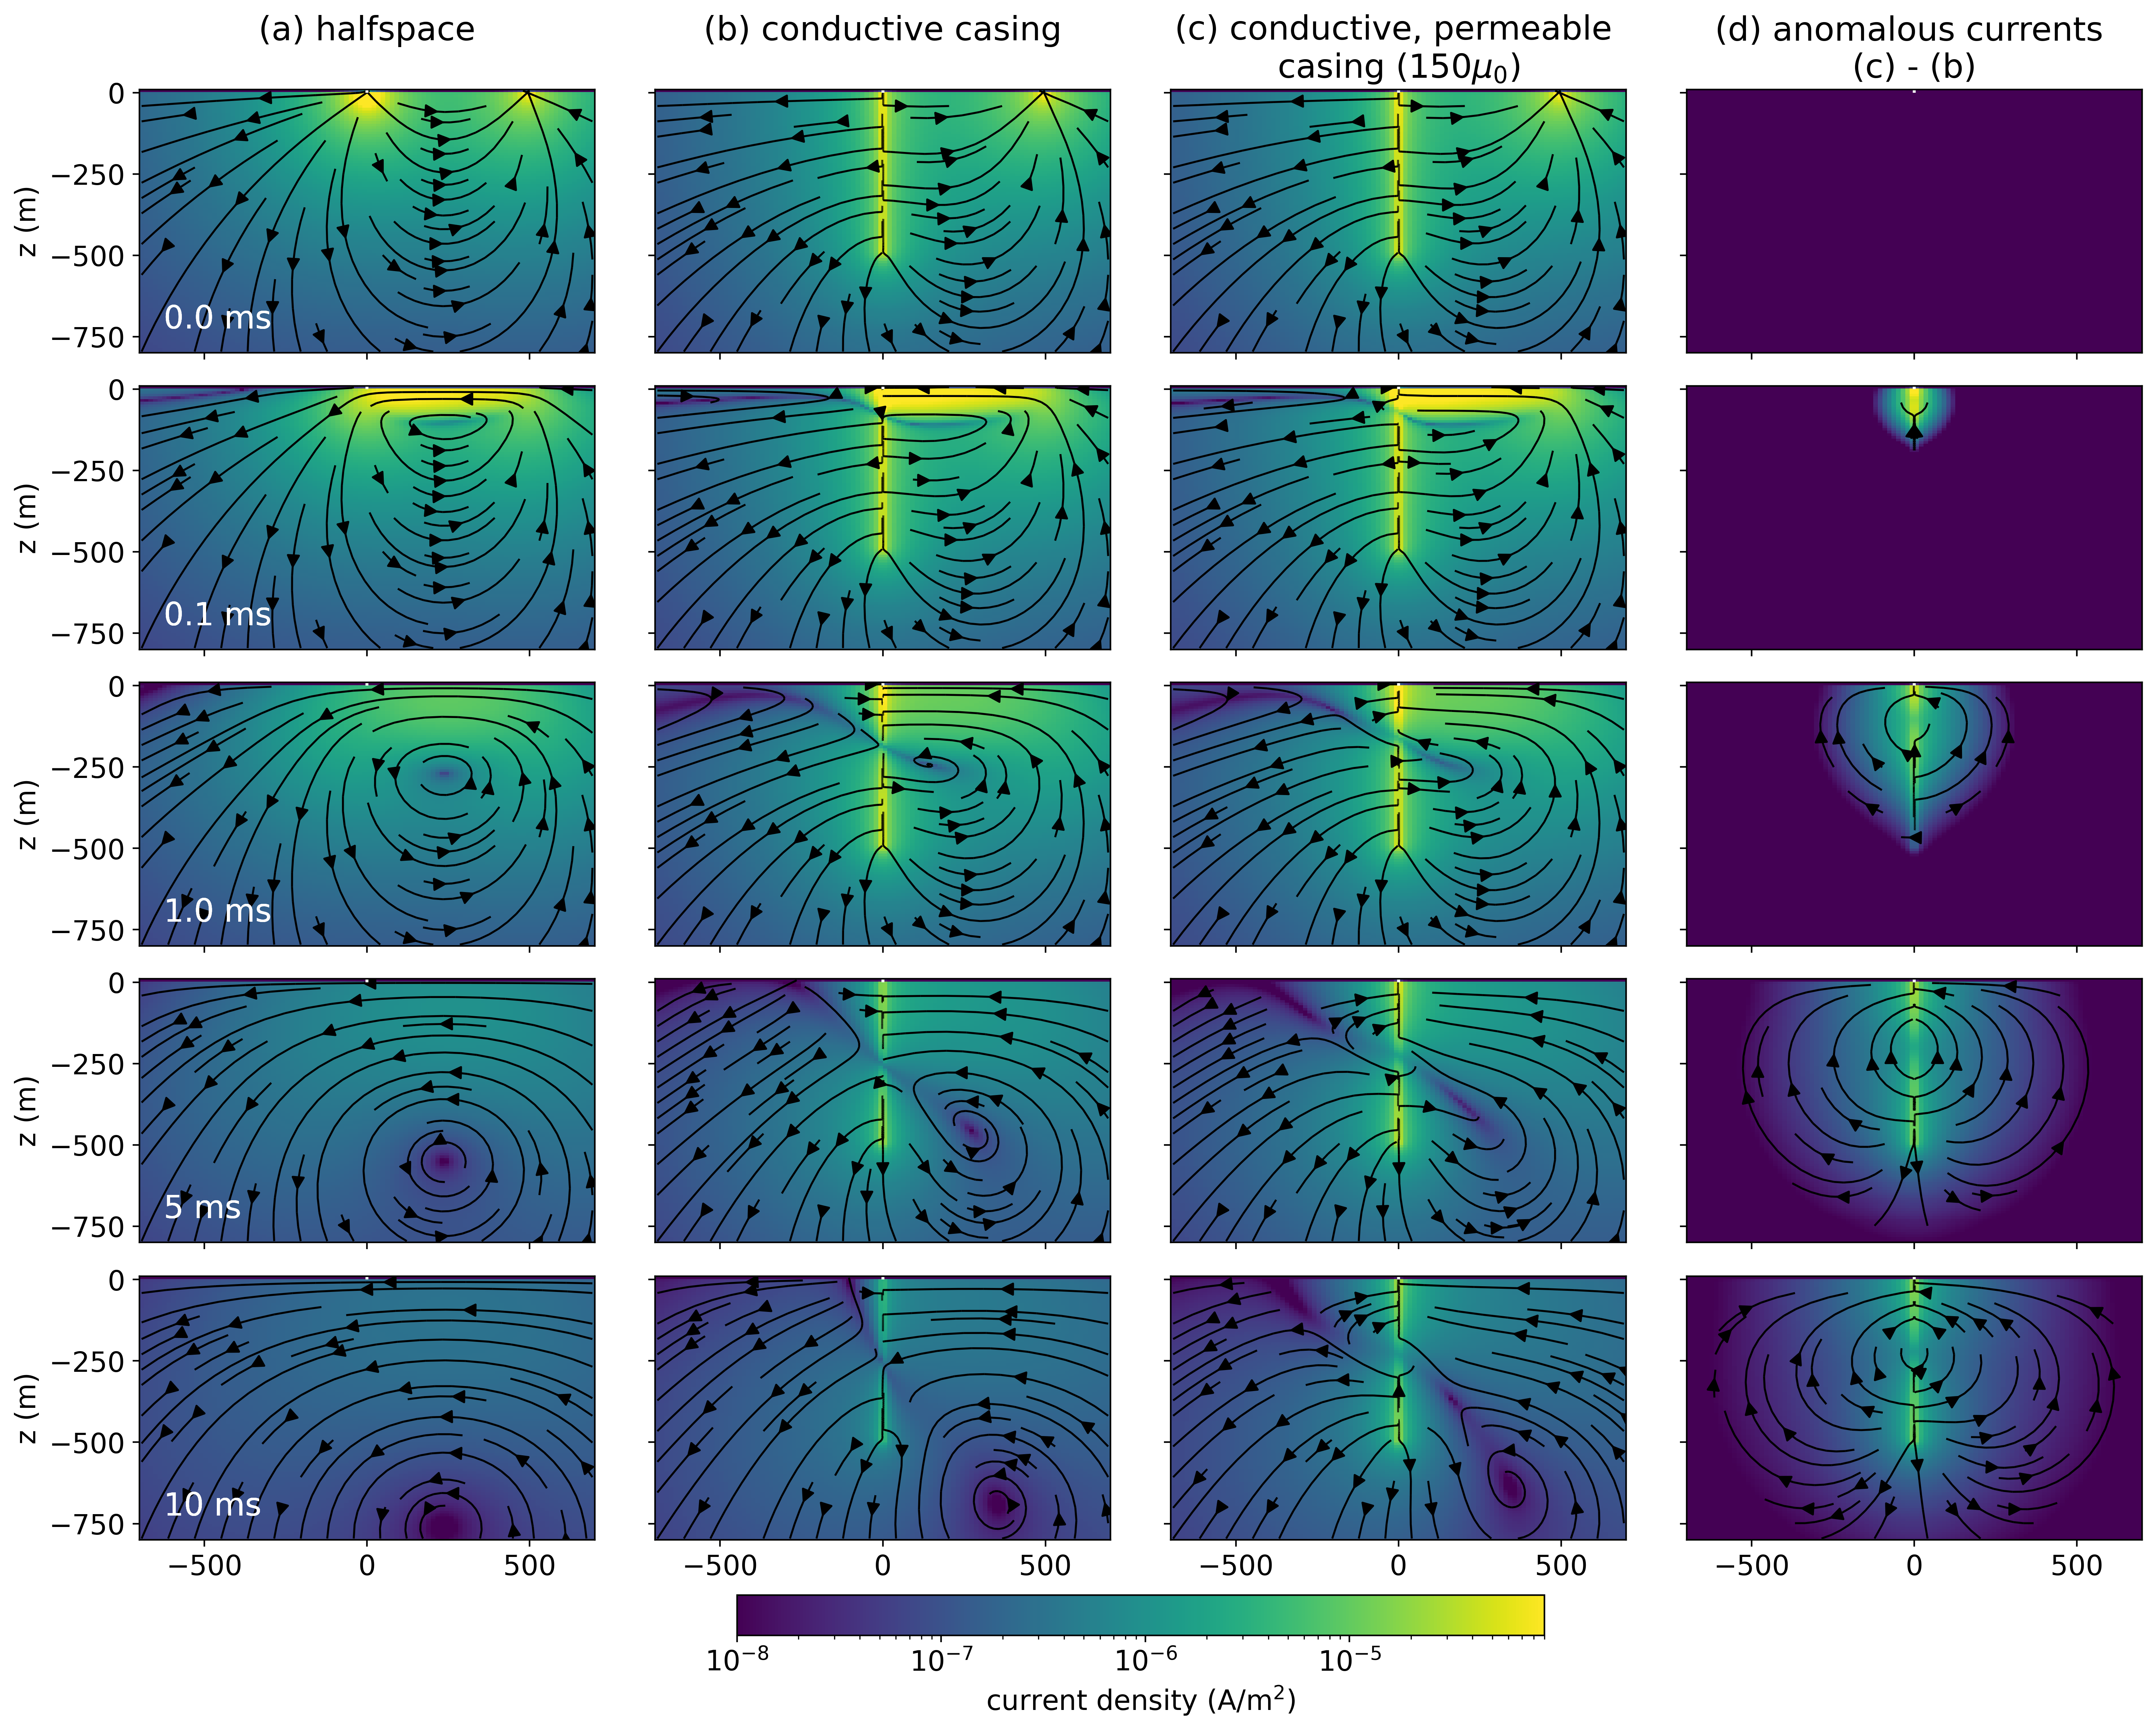
\includegraphics[width=\textwidth]{figures/tdem-cross-section-currents.png}
    \end{center}
\caption{Cross sections showing the current density through time for a time domain EM experiment over (a) a half-space, (b) a conductive well ($5\times10^6$ S/m, $\mu_0$), and (c) a conductive, permeable well ($5\times10^6$ S/m, $150\mu_0$). The panel on the right shows (d) the difference between the conductive, permeable well and the conductive well. The threshold for the streamplot arrows is the same as the colorbar minimum ($10^{-8}$A/m$^2$)
}
\label{fig:tdem-cross-section-currents}
\end{figure}



